\documentclass[a4paper]{jsarticle}
\usepackage[dvipdfmx]{graphicx}
\usepackage{amsmath}
\usepackage{bm}
\renewcommand{\thesection}{第\arabic{section}問}
\renewcommand{\thesubsection}{(\arabic{subsection})}
\renewcommand{\thesubsubsection}{(\alph{subsubsection})}
\begin{document}

\title{2022分野3}
\author{nakao}
\maketitle

\section{}
\subsection{}
式[2]において
$\frac{\partial v}{\partial t} = 0, i_f = 0$
として、
\begin{equation}
  \frac{\partial}{\partial x}
  \left(\frac{v^2}{2g} + h + z\right) = 0
\end{equation}
となる。

\subsection{}
気持ち悪いので
$i_0 = -\frac{\partial z}{\partial x}$
として進めます。出題ミス??
\subsubsection{}
エネルギー保存則は、
\begin{equation}
  \frac{\partial E_s}{\partial x} = i_0 - i_f
\end{equation}
と表される。等流のとき$h = h_0$で一定であるから
\begin{align}
  \frac{\partial E_s}{\partial x}
  &= \frac{\partial}{\partial x}
  \left(\frac{q^2}{2 g h_0^2} + h_0\right)
  = 0 \\
  i_f &= n^2 h_0^{-\frac{4}{3}} \left(\frac{q}{h_0}\right)^2
  = n^2 q^2 h_0^{-\frac{10}{3}}
\end{align}
となり、これらを式(2)に代入すると、
\begin{equation}
  h_0 = \left(\frac{n^2 q^2}{i_0}\right)^{\frac{3}{10}}
\end{equation}
が得られる。

\subsubsection{}
式(5)より
\begin{equation}
  \frac{\partial E_s}{\partial x}
  = i_0 - i_f
  = i_0 \left\{1 - \left(\frac{h_0}{h}\right)^{\frac{10}{3}}\right\}
\end{equation}
が成り立つから、
$h > h_0$のとき、$\frac{\partial E_s}{\partial x} > 0$であり、
また$h < h_0$のとき、$\frac{\partial E_s}{\partial x} < 0$となる。

\subsubsection{}
$h = h_0$で一定のとき、満たすべき条件は
\begin{equation}
  \mathrm{Fr}^2 = \frac{q^2}{g h_0^3} > 1
\end{equation}
であり、式[5]を代入して計算すると
\begin{equation}
  i_0 > n^2 q^{-\frac{2}{9}} g^{\frac{10}{9}}
\end{equation}
を得る。\par
以下、$\frac{\partial h}{\partial x} \neq 0$の場合を考える。
\begin{equation}
  \frac{\partial E_s}{\partial x}
  = \frac{\partial}{\partial x}
  \left(\frac{q^2}{2 g h^2} + h\right)
  = (1 - \mathrm{Fr}^2) \frac{\partial h}{\partial x}
\end{equation}
であり、式(2)とManningの式
$i_f = n^2 q^2 h_0^{-\frac{10}{3}}$
より、
\begin{equation}
  (1 - \mathrm{Fr}^2) \frac{\partial h}{\partial x}
  = i_0 - n^2 q^2 h_0^{-\frac{10}{3}}
\end{equation}
となる。したがって、満たすべき条件は、
\begin{equation}
  1 - \mathrm{Fr}^2 =
  \frac{i_0 - n^2 q^2 h_0^{-\frac{10}{3}}}{\frac{\partial h}{\partial x}} < 0
\end{equation}
と表せる。
$\frac{\partial h}{\partial x}$の符号に分けて記述すると、
\begin{equation}
  \begin{cases}
    i_0 < n^2 h^{-\frac{10}{3}} q^2
    & \left(\frac{\partial h}{\partial x} > 0\right) \\
    i_0 > n^2 h^{-\frac{10}{3}} q^2
    & \left(\frac{\partial h}{\partial x} < 0\right) \\
  \end{cases}
\end{equation}
である。

\subsubsection{}
式(6),(9)より、
\begin{equation}
  (1 - \mathrm{Fr}^2) 
  = i_0 \left\{1 - \left(\frac{h_0}{h}\right)^{\frac{10}{3}}\right\}
\end{equation}
が成り立つ。これより、
\begin{equation}
  \frac{\partial h}{\partial x}
  = i_0 \frac{1 - \left(\frac{h_0}{h}\right)^{\frac{10}{3}}}{1 - \mathrm{Fr}^2}
\end{equation}
である。ここで、射流の条件を常に満たすことを仮定しているため、
$1 - \mathrm{Fr}^2 < 0$である。\par
したがって、$h > h_0$のとき
$\frac{\partial h}{\partial x} < 0, \frac{\partial h}{\partial x} \xrightarrow{h \to h_0} 0$
が成り立つ。また、$h < h_0$のとき、
$\frac{\partial h}{\partial x} > 0, \frac{\partial h}{\partial x} \xrightarrow{h \to h_0} 0$
が成り立つ。

\subsection{}
式[3],[4]より
\begin{equation}
  \left(c - \frac{\mathrm{d} q}{\mathrm{d} h}\right)
  \frac{\partial h}{\partial x} = 0
\end{equation}
が成り立ち、波が進行するときに
$\frac{\partial h}{\partial x} \neq 0$
であるとすれば、
\begin{equation}
  c = \frac{\mathrm{d} q}{\mathrm{d} h}
  = \frac{\mathrm{d}}{\mathrm{d} h} (v h)
  = \frac{\mathrm{d}}{\mathrm{d} h} \left(n^{-1} h^{\frac{5}{3}} i_0^{\frac{1}{2}}\right)
  = \frac{5}{3} v
\end{equation}
である。

\subsection{}
Manningの式と式(16)より
\begin{equation}
  h = \left(v n i^{-\frac{1}{2}}\right)^{\frac{3}{2}}
  = \left(\frac{3}{5} c n i^{-\frac{1}{2}}\right)^{\frac{3}{2}}
\end{equation}
である。ここに、
$c = 1 \, \mathrm{km} / 200 \, \mathrm{s} = 5 \,\mathrm{m s^{-1}}$,
$n = 0.025 \, \mathrm{m^{-\frac{1}{3}} s}$,
$i_0 = 1/900$を代入すると、
$h = 3.375 \, \mathrm{m}$が得られる。

\subsection{}
\subsubsection{}
kinematic waveの運動方程式は、
$-i_0 + i_f = 0$であり、diffusion waveの運動方程式は、
$\frac{\partial h}{\partial x} - i_0 + i_f = 0$である。
それぞれにManningの式
$v = n^{-1} h^{\frac{2}{3}} i_0^{\frac{1}{2}}$
を代入すると、それぞれの流量は、
\begin{align}
  q_{kine} &= n^{-1} h^{\frac{5}{3}} i_0^{\frac{1}{2}} \\
  q_{diff} &= n^{-1} h^{\frac{5}{3}} \left(i_0^{\frac{1}{2}} - \frac{\partial h}{\partial x}\right)
\end{align}
と表される。したがって、水深-流量の関係の概略図は図1の通り。
diffusion waveでは、水深の勾配に応じて、kinematic waveからの流量がずれる。
\begin{figure}[htb]
  \centering
  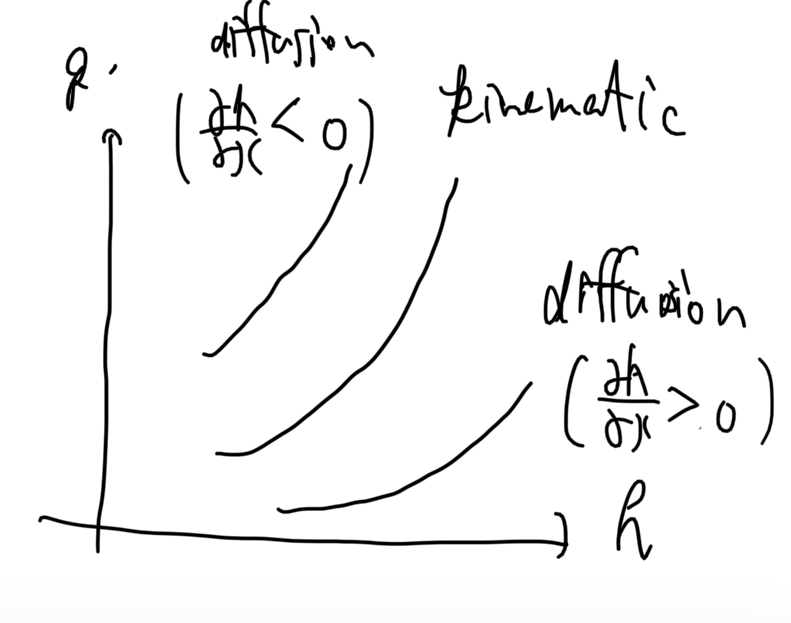
\includegraphics[width=0.3\hsize]{fig1.png}
  \caption{水深-流量の関係の概略図}
\end{figure}

\subsubsection{}
小河川における大河川との合流部など、下流側の水位が高くなっている場所。
下流側からの逆流により、流量のキャパシティが減少する。

\subsection{}
災害規模と被害規模の関係を推察することができるようになり、
防災の効果が検証しやすくなる。費用対効果の高い施策が行うための意思決定に役立つ。
市民はどのような災害に対して居住地域が大きな被害を受けるかを確認し、
自身がどのタイプの災害を恐れるべきか理解できる。

\section{}

\end{document}

